
\plain{Answers: Organic Best Of vs Bandit Best Of}




\begin{frame}[fragile]
  \frametitle{Answer Q1 Histogram of product popularity}
\begin{small}
\begin{verbatim}
  clicks = np.zeros(NumberOfProducts)
  bandits = data[data['z'] == 'bandit']
  for product_id in range(NumberOfProducts):
      actions = bandits[bandits['a'] == product_id]
      clicks[product_id] = np.sum(actions[actions['c'] == 1]['c'])
      
  print("Clicks: ", clicks)
  
  _, ax = plt.subplots()
  ax.set_title('Histogram of Clicks per Product')
  
  ax.bar(range(NumberOfProducts), clicks)
  plt.show()
\end{verbatim}
\end{small}
\end{frame}


\begin{frame}[fragile]
  \frametitle{Answer Q2 Non-personalized CTR}
\begin{tiny}
\begin{verbatim}
  from scipy.stats.distributions import beta

  clicks = np.zeros(NumberOfProducts)
  impressions = np.zeros(NumberOfProducts)
  lower_errors = np.zeros(NumberOfProducts)
  upper_errors = np.zeros(NumberOfProducts)
  bandits = data[data['z'] == 'bandit']
  for product_id in range(NumberOfProducts):
      actions = bandits[bandits['a'] == product_id]
      clicks[product_id] = np.sum(actions[actions['c'] == 1]['c'])
      impressions[product_id] = sum(actions['a']==product_id)
\end{verbatim}
\end{tiny}
\end{frame}

\begin{frame}[fragile]
  \frametitle{Answer Q3 Best of CTR}
\begin{verbatim}
  top_ctr_item = np.argmax(clicks/impressions)
\end{verbatim}
\end{frame}


\begin{frame}[fragile]
  \frametitle{Answer Q4 most views}
\begin{verbatim}
  top_viewed_item = np.argmax(views)
\end{verbatim}
\end{frame}




\begin{frame}[fragile]
  \frametitle{}
  \begin{small}
\begin{verbatim}
data = deepcopy(env).generate_logs
        (ABTestNumberOfUsers, agent=organic_counter_agent)
\end{verbatim}
\end{small}
\end{frame}




\begin{frame}
\frametitle{Organic Best-Of vs Bandit Best-Of}

As the logging policy chose its actions uniformly at random, we can see that all items were recommended roughly the same number of times.

\begin{figure}[h!]
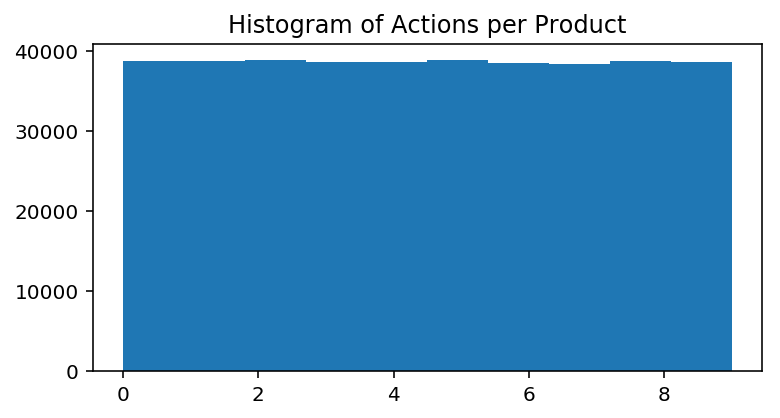
\includegraphics[scale=0.4]{images/organic_bestof0.png}
\centering
\label{motex1}
\end{figure}
\end{frame}

\begin{frame}
\frametitle{Organic Best-Of vs Bandit Best-Of}

We can examine the click through rate of each action under this policy, we see that action 5, 2 and 9 have high click through rates.

\begin{figure}[h!]
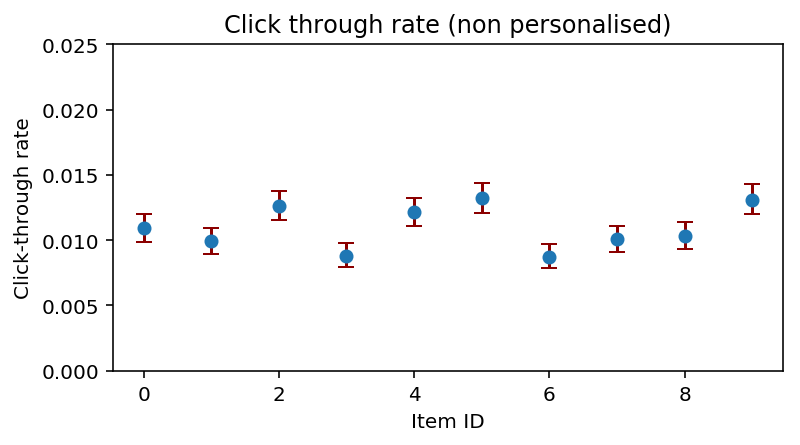
\includegraphics[scale=0.4]{images/organic_bestof1.png}
\centering
\label{motex1}
\end{figure}
\end{frame}

\begin{frame}
\frametitle{Organic Best-Of vs Bandit Best-Of}


\begin{figure}[h!]

  We can also examine which items are organically the most popular, this time we see that item 4 and item 9 are the most popular.

  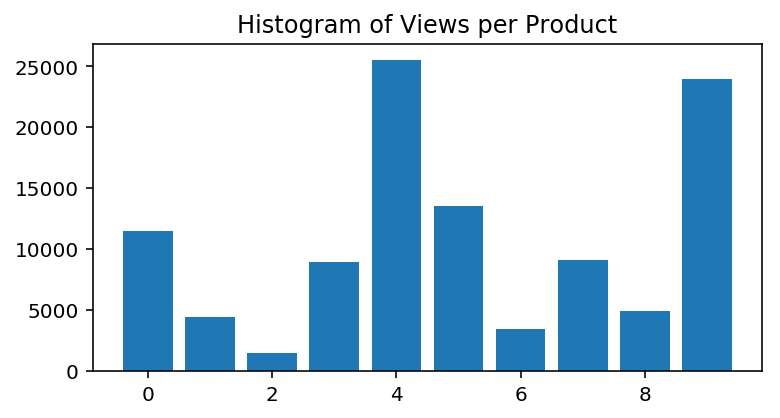
\includegraphics[scale=0.4]{images/organic_bestof2.png}
\centering
\label{motex1}
\end{figure}
\end{frame}

\begin{frame}
\frametitle{Organic Best-Of vs Bandit Best-Of}

If we plot popularity vs non-personalized click through rate we see some kind of relationship, but the correlation is noisy.


\begin{figure}[h!]
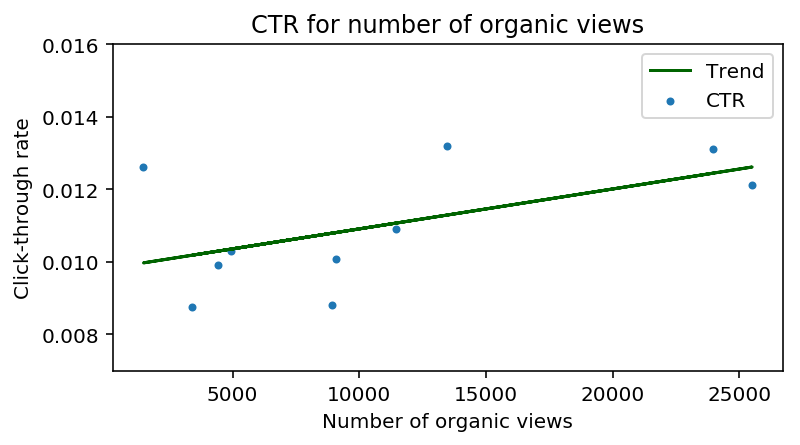
\includegraphics[scale=0.4]{images/organic_bestof3.png}
\centering
\label{motex1}
\end{figure}
\end{frame}

\begin{frame}
\frametitle{Organic Best-Of vs Bandit Best-Of}

A bandit best-of agent always recommends the highest ctr product (product 5).  An organic best-of always recommends the most frequently viewed product (product 4).  A simulated AB test shows using the bandit best-of yields a better result.

\end{frame}

\begin{frame}
\frametitle{Organic Best-Of vs Bandit Best-Of}
  
\begin{figure}[h!]
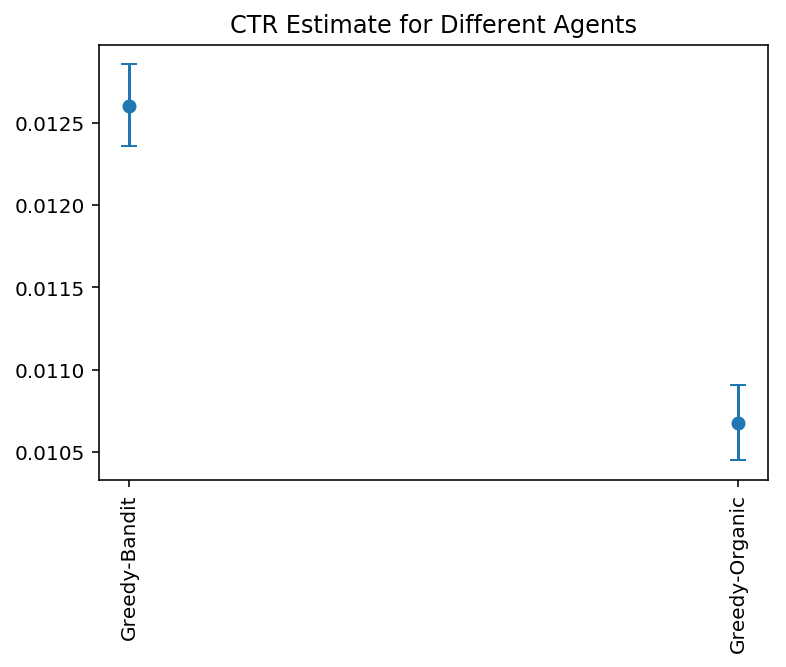
\includegraphics[scale=0.4]{images/bestof.png}
\centering
\label{motex1}
\end{figure}

\pause
Personalization of course will result in a better result still.
\end{frame}


\plain{Answers: Evaluate an organic agent using the Bandit Signal}



\begin{frame}[fragile]
  \frametitle{Answer}
\begin{tiny}  
\begin{verbatim}
def observe(self, observation):
  for session in observation.sessions():
      self.user_embedding += self.embeddings[session['v'],:]
      self.history_length += 1

def act(self, observation, reward, done):
  """Act method returns an Action based on current observation and past history"""
  self.observe(observation)
  next_item_score = np.matmul(self.embeddings,self.user_embedding/self.history_length)

  action = np.argmax(next_item_score)        
  prob = np.zeros_like(next_item_score)
  prob[action]=1.0
  return {
      **super().act(observation, reward, done),
      **{
          'a': action,
          'ps': 1.0,
          'ps-a': prob,
      },
  }
\end{verbatim}
\end{tiny}
\end{frame}

\plain{Answers Evaluate on Bandit}







\begin{frame}
  \frametitle{Evaluate an organic model using Bandit Feedback}

  Methods like word2vec and SVD can be used to produce a low rank factorization of a matrix of co-counts.  Imagine we have 500 products and we have observed the co-counts on the right, the matrix on the left can produce a good reconstruction (perhaps better than the original as it can fill in missing signal).  It also uses less parameters, which has both computational and statistical advantages.

  You could also use deep learning (see modules 1 and 2 of our course)

  \begin{figure}[h!]
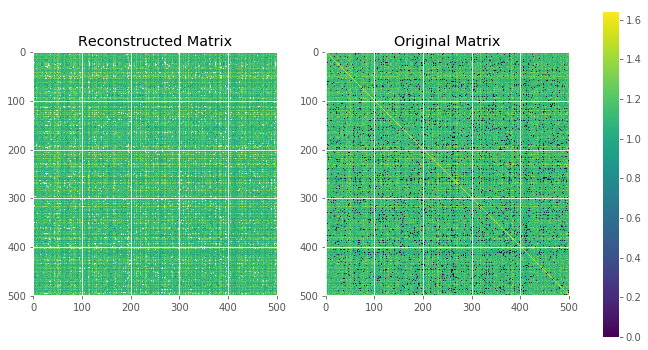
\includegraphics[scale=0.4]{images/evalorganicwithbandit0.png}
\centering
\label{motex1}
\end{figure}
\end{frame}


\begin{frame}
  \frametitle{Evaluate an organic model using Bandit Feedback}
\begin{figure}[h!]
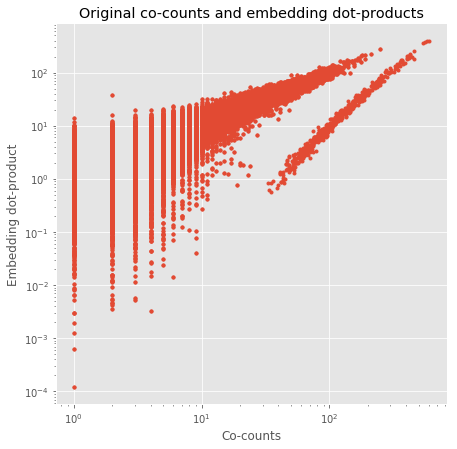
\includegraphics[scale=0.4]{images/evalorganicwithbandit1.png}
\centering
\label{motex1}
\end{figure}
\end{frame}


\begin{frame}
  \frametitle{Evaluate an organic model using Bandit Feedback}

  For such an organic method, a standard metric is hitrate-at-5 (HR@5) also called Recall@5 or Precision@5.
\begin{figure}[h!]
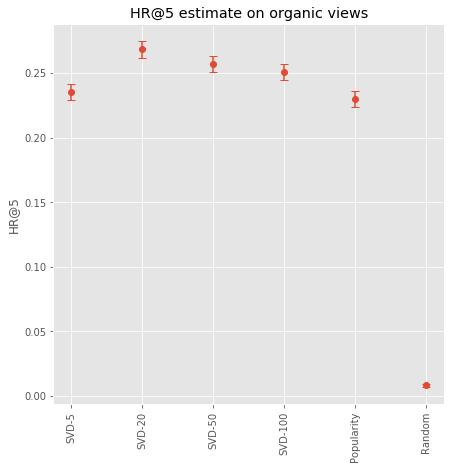
\includegraphics[scale=0.4]{images/evalorganicwithbandit2.png}
\centering
\label{motex1}
\end{figure}
\end{frame}

\begin{frame}
  \frametitle{Evaluate an organic model using Bandit Feedback: IPS evaluation}

Hit-rate is a purely organic measure that is available offline and is seen in many recommender systems papers...  \pause but it is a purely organic metric, it doesn't predict performance at AB test time, at least not explicitly.

\pause

Can we change to an offline measure that predicts the result of an AB test?

\pause

Imagine the past policy is randomized, i.e. with some probability it will choose any action for a given user.  \pause Random isn't the same as uniform and the policy typically will not be uniformly random. \pause \emph{Why?} \pause ... still, a uniformly random logging policy is an interesting thought experiment or reference.

\end{frame}

\begin{frame}
  \frametitle{Evaluate an organic model using Bandit Feedback: IPS evaluation}

The central idea of an inverse propensity score is that we evaluate a new policy using the logs of an old policy.  \pause We identify times in history where the new policy would make the same recommendation as the old policy, we then look at the contribution of the reward and how probable the policy is to take this action. 

\[
\text{CTR}_{\pi_t}(\mathcal{L}) = \frac{1}{|\mathcal{L}|}\sum_{(a,x,c) \in \mathcal {L}} c \frac{\pi_t(a|x)}{\pi_l(a|x)}
\]

\end{frame}


\begin{frame}
  \frametitle{Evaluate an organic model using Bandit Feedback}
\begin{figure}[h!]
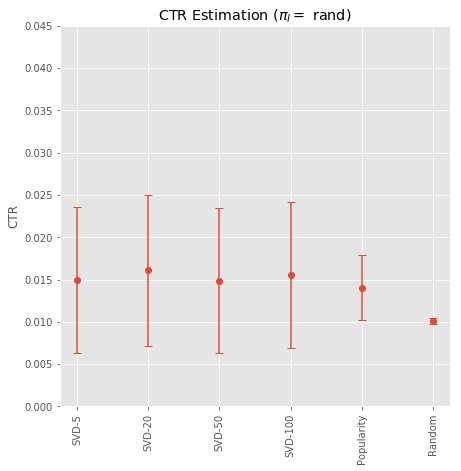
\includegraphics[scale=0.4]{images/evalorganicwithbandit3.png}
\centering
\label{motex1}
\end{figure}
\end{frame}

\begin{frame}
  \frametitle{Evaluate an organic model using Bandit Feedback}
\begin{figure}[h!]
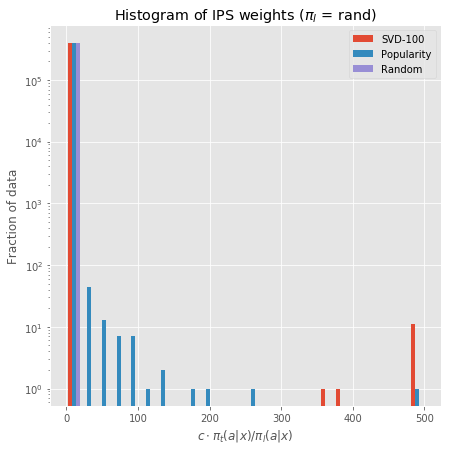
\includegraphics[scale=0.4]{images/evalorganicwithbandit4.png}
\centering
\label{motex1}
\end{figure}
\end{frame}

\begin{frame}
  \frametitle{Evaluate an organic model using Bandit Feedback}
\begin{figure}[h!]
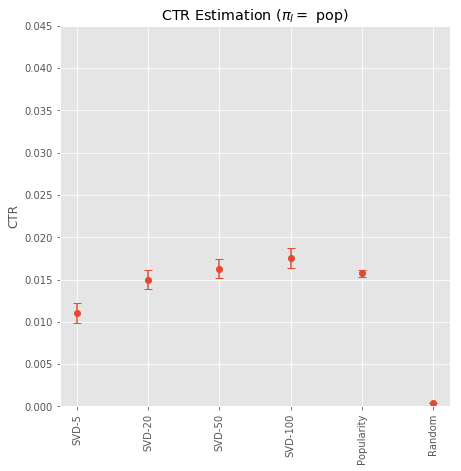
\includegraphics[scale=0.4]{images/evalorganicwithbandit5.png}
\centering
\label{motex1}
\end{figure}
\end{frame}

\begin{frame}
  \frametitle{Evaluate an organic model using Bandit Feedback}
\begin{figure}[h!]
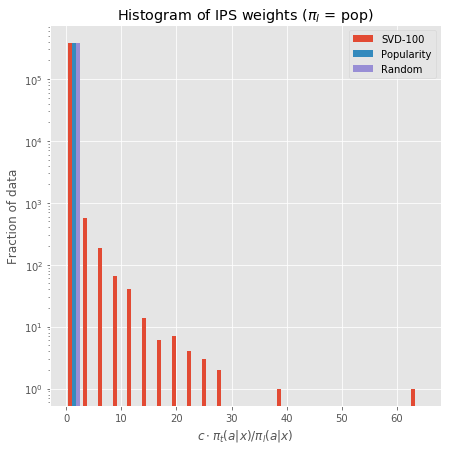
\includegraphics[scale=0.4]{images/evalorganicwithbandit6.png}
\centering
\label{motex1}
\end{figure}
\end{frame}


\begin{frame}
  \frametitle{Evaluate an organic model using Bandit Feedback: Simulated A/B-Test Results}
\begin{figure}[h!]
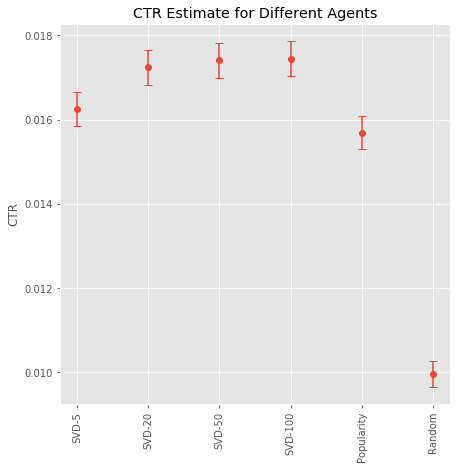
\includegraphics[scale=0.4]{images/evalorganicwithbandit7.png}
\centering
\label{motex1}
\end{figure}
\end{frame}
